\chapter{Aufgabe 9}
\section{Algorithmus zur Bestimmung der Samplingrate}
Um die Samplingrate der Aufnahme des Oszilloskops zu bestimmen, sollte zunächst die Periodendauer T berechnet werden.
Da die Frequenz f hier bekannt ist geht dies über die Beziehung T = $\frac{1}{T}$ .
Nun muss die Anzahl N der Samples pro Periode festgestellt werden.
Dazu muss die Anzahl der Messwerte zwischen zwei Minima bestimmt werden.
Anschließend kann die Samplingrate SR mit der Beziehung SR = $\frac{N}{T}$ berechnet werden.
Fasst man beide Formeln zusammen führt dies zu der Beziehung SR = N $\cdot$ f .
Der Algorithmus ist als Ablaufdiagramm in Abbildung \ref{algo1} zusehen. \par 

\begin{figure}[h]
	\centering
	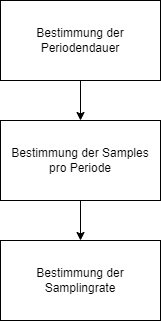
\includegraphics[scale=0.5]{Images/aufgabe9_algo1.png}
	\caption{Ablaufdiagramm des ersten Algorithmus der Aufgabe9}
	\label{algo1}
\end{figure}

\section{Algorithmus zur Bestimmung der Frequenz}
Da in der Aufgabe keine Samplingrate angegeben ist, nehme ich an das diese aus dem ersten Algorithmus bestimmte Samplingrate verwendet werden soll.
Zunächst muss die Anzahl der Messwerte pro Periode bestimmt werden. 
Dazu wird wieder eine Periode mithilfe der Minima festgestellt werden un die Messwerte zwischen zwei Minima gezählt. 
Anschließend kann aus der Beziehung SR = $\frac{N}{T}$ , durch Umstellung, die Beziehung T = $\frac{N}{SR}$ gebildet werden. 
Somit erhalten wir die Periodendauer T und können daraus die Frequenz mit der Formel f = $\frac {1}{T}$ berechnen.
Mann kann diese Formeln auch zusammenfassen zu der Beziehung f = $\frac{SR}{N}.$
Dieser Algorithmus ist in Abbildung \ref{algo2} dargestellt.\par

\begin{figure}[h]
	\centering
	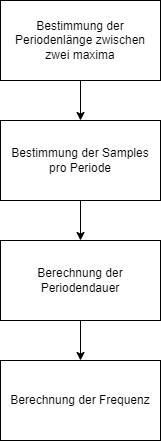
\includegraphics[scale=0.5]{Images/aufgabe9_algo2.png}
	\caption{Ablaufdiagramm des zweiten Algorithmus der Aufgabe 9}
	\label{algo2}
\end{figure}

\section{Algorithmus zur Bestimmung der Frequenz einer Rechteckspannung}
Um die Frequenz der Rechteckspannung zu bestimmen, kann wieder die bereits ermittelte Samplingrate verwendet werden. 
Somit muss wieder die die Anzahl der Messwerte pro Periode bestimmt werden.
Als Periodenbeginn wird der beginn des Maximalwert bis nächsten beginn des Maximalwert festgelegt.
Nun muss die Anzahl der Messwerte dazwischen gezählt werden,
Anschließend kann mit der Formel T = $\frac{N}{SR}$ und der Formel f = $\frac{1}{T}$ die Frequenz bestimmt werden.
Fasst man diese wieder zusammen führt dies zu der Formel f = $\frac{SR}{N}$ .
In der Abbildung \ref{algo3} ist das Ablaufdiagramm des Algorithmus dargestellt.\par

\begin{figure}[h]
	\centering
	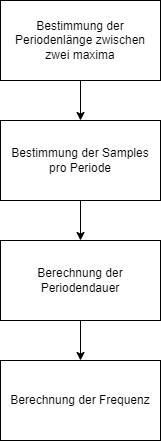
\includegraphics[scale=0.5]{Images/aufgabe9_algo3.png}
	\caption{Ablaufdiagramm des dritten Algorithmus der Aufgabe 9}
	\label{algo3}
\end{figure}

\section{Repo}
In diesem Repo auf auf Gitlab befindet sich der Programmierteil der Aufgabe 9.
In diesem Repo befinden sich die Implementierungen der Algorithmen aus Aufgabe 9.
Diese dienen dazu die Samplingrate einer Aufnahme einer Oszilloskop Kurve bei bekannter Frequenz zu bestimmen und die Frequenz bei bekannter Samplingrate zu bestimmen.\par

\href{https://gitlab.thga.de/daniel.krueger/pruefung_sose_2023_aufgabe_9_algorithmen}{\textbf{LINK}}
